\section{Method}
\label{sec:method}
Given queries $Q \in \mathbb{R}^{n \times d}$ and keys partitioned into blocks
$K_1, \dots, K_m$, a router scores each block and keeps the top $k$:
\begin{equation}
  r_i = \operatorname{top-}k\big(\operatorname{softmax}(q_i W_r)\big).
\end{equation}
We train a transformer with twelve layers for three days on 8~GPUs.
Hyperparameters were chosen by intuition.

\begin{figure}[t]
  \centering
  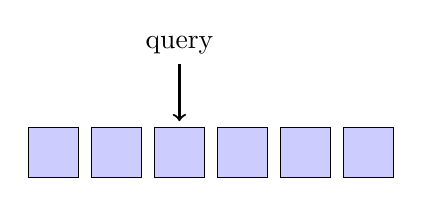
\begin{tikzpicture}[scale=0.8]
    \foreach \x in {0,...,5} \draw[fill=blue!20] (\x,0) rectangle (\x+0.8,0.8);
    \draw[->,thick] (2.4,1.8) -- (2.4,0.9);
    \node at (2.4,2.1) {query};
  \end{tikzpicture}
  \caption{The router sends each query to a few key blocks.}
\end{figure}
